\documentclass[border=3mm]{standalone}

\usepackage{xcolor}

\definecolor{palesilver}{rgb}{0.79, 0.75, 0.73}
\definecolor{silver}{rgb}{0.75, 0.75, 0.75}
\definecolor{goldenbrown}{rgb}{0.6, 0.4, 0.08}
\definecolor{glaucous}{rgb}{0.38, 0.51, 0.71}
\usepackage{tikz}
\usetikzlibrary{shapes,decorations,shadows}

\usetikzlibrary{calc}


\usetikzlibrary{decorations.text}



\begin{document}


\tikzset{paint/.style={ draw=#1!50!black, fill=#1!50 },
    decorate with/.style=
    {decorate,decoration={shape backgrounds,shape=#1,shape size=2mm}}}




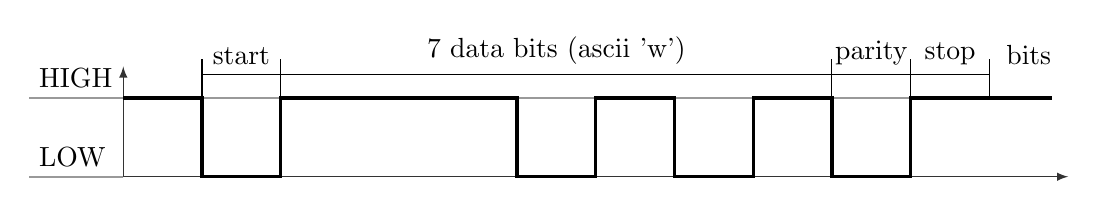
\begin{tikzpicture} 
  %ticks
  \draw[thick,color=black!40] (0,0) -- (-1.2,0) node[anchor=south west,color=black] {LOW};
  \draw[thick,color=black!40] (11,1) -- (-1.2,1)     
  (-1.2,1) node[anchor=south west,color=black] {HIGH};  
  %axis
	\draw[-latex,color=black!80] (0,0) -- coordinate (x axis mid) (12,0);
    \draw[-latex,color=black!80] (0,0) -- coordinate (y axis mid) (0,1.4);
  % signal w
  \draw[very thick] (0,1) -- (1,1) -- (1,0) -- (2,0) -- (2,1) -- (5,1) -- (5,0) -- (6,0) -- (6,1) -- (7,1) -- (7,0) -- (8,0) -- (8,1) -- (9,1) -- (9,0) -- (10,0) -- (10,1) -- (11.8,1);   
  % character bits
  \draw (2,1) -- (2,1.5);
  \draw (9,1) -- (9,1.5);
  \draw[] (2,1.3) -- coordinate (c axis mid) (9,1.3);
  \node[anchor=south] at (c axis mid) {7 data bits (ascii 'w')};
  % start and parity bits
  \draw (1,1) -- (1,1.5);
  \draw[] (1,1.3) -- coordinate (start axis mid) (2,1.3);
  \node[anchor=south] at (start axis mid) {start}; 
  \draw[] (9,1.3) -- coordinate (parity axis mid) (10,1.3);
  \node[anchor=south] at (parity axis mid) {parity}; 
  % stop bits
  \draw (10,1) -- (10,1.5);
  \draw (11,1) -- (11,1.5);
  \draw[] (10,1.3) -- coordinate (stop axis mid) (11,1.3);
  \node[anchor=south] at (stop axis mid) {stop};
  % bits
  \node[anchor=south] at (11.5,1.3) {bits}; 
\end{tikzpicture}


\end{document}